\chapter{Chapitre 1 : Cadre du projet et étude de l'existant}\label{chap1}

\section{Introduction}

La gestion des dossiers médicaux est un domaine où la confidentialité, l'intégrité et la traçabilité des données sont aussi importantes que la disponibilité du service. Les systèmes classiques reposent sur une base relationnelle unique et sur des journaux d'audit stockés dans la même infrastructure : une altération des données peut donc rester indétectable si le journal est lui aussi modifié. Le projet \textbf{MedChain} propose une architecture où chaque événement clinique sensible est chiffré puis résumé par une empreinte inscrite dans une chaîne de blocs immuable, elle-même ancrée sur un registre EVM local.

Ce premier chapitre présente le contexte, la problématique, les objectifs, une étude critique des solutions existantes et la méthodologie de gestion de projet retenue.

\section{Organisme d'accueil et contexte}

Le projet est réalisé au sein de \textbf{Tekup University}, établissement d'enseignement supérieur en ingénierie logicielle. La Figure \ref{fig:logo_tekup} présente son identité visuelle.

\begin{figure}[H]
\centering

\includegraphics[width=0.3\textwidth]{Images/tek_up_logo.jpg}
\caption{Logo de Tekup University}
\label{fig:logo_tekup}
\end{figure}

Le travail s'inscrit dans une démarche de conception sécurisée : les données personnelles de santé sont traitées selon le principe de moindre privilège, et chaque accès sensible fait l'objet d'une écriture dans un journal d'audit.

\section{Problématique}

La question centrale est la suivante : \textit{comment garantir qu'un dossier médical partagé entre un patient et un médecin n'a pas été altéré, tout en préservant la confidentialité de son contenu et en offrant une preuve vérifiable de son historique ?}

Trois contraintes structurent la réponse :

\begin{itemize}
    \item \textbf{Confidentialité :} le contenu des événements cliniques ne doit jamais être stocké en clair dans la base ni exposé par l'API.
    \item \textbf{Intégrité :} toute modification d'un événement déjà enregistré doit être détectable, y compris si l'attaquant accède à la base de données.
    \item \textbf{Traçabilité :} les actions sensibles (connexion, consultation, autorisation, refus) doivent être journalisées et consultables par l'administrateur.
\end{itemize}

\section{Solution proposée}

MedChain est une application web composée d'une interface React, d'une API Django REST, d'une passerelle Nginx et de services d'infrastructure. La Figure \ref{fig:contexte} donne la vue d'ensemble du système et de ses acteurs.

\begin{figure}[H]
\centering
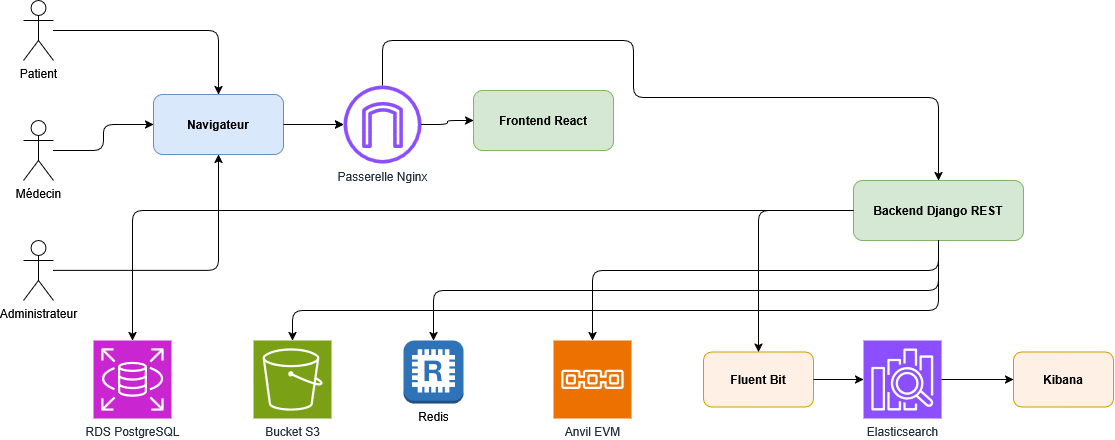
\includegraphics[width=\textwidth]{Chapters/1/images/01-contexte-systeme.png}
\caption{Vue d'ensemble du système MedChain}
\label{fig:contexte}
\end{figure}

Les fonctionnalités principales sont :

\begin{itemize}
    \item l'authentification par jeton de session et l'authentification Google (web et mobile) ;
    \item la distinction des rôles patient, médecin et administrateur ;
    \item la gestion des rendez-vous et des dossiers médicaux ;
    \item la demande, l'activation, l'échec ou la clôture d'un épisode de traitement ;
    \item le chiffrement des événements cliniques par une clé de données propre à l'épisode ;
    \item l'ancrage des empreintes de blocs sur une chaîne EVM locale ;
    \item la supervision des comptes, des journaux d'audit et des alertes de sécurité.
\end{itemize}

\section{Étude de l'existant}

\subsection{Dossiers médicaux classiques}

Les systèmes de gestion de dossiers médicaux offrent généralement le stockage structuré des consultations, des prescriptions et des résultats d'analyses. Leurs limites sont la centralisation des données et l'absence de preuve d'intégrité indépendante du système lui-même.
\newline 
\newline 
\newline 


\subsection{Registres distribués et ancrage}

Les registres distribués permettent de publier une empreinte immuable d'un document sans publier le document lui-même. Cette propriété est adaptée au domaine médical : on conserve le contenu chiffré dans la base et on ancre uniquement son empreinte. MedChain adopte ce modèle avec une chaîne EVM locale (Anvil) pour la phase de démonstration.

\subsection{Synthèse}

\begin{table}[H]
\centering
\renewcommand{\arraystretch}{1.3}
\begin{tabular}{|l|p{4cm}|p{4cm}|}
\hline
\textbf{Critère} & \textbf{Système classique} & \textbf{MedChain} \\
\hline
Confidentialité & Accès contrôlé & Chiffrement par épisode \\
\hline
Intégrité & Journal interne & Chaîne de blocs et ancrage \\
\hline
Traçabilité & Journaux applicatifs & Journaux + événements immuables \\
\hline
Stockage & Base unique & RDS pour les données, S3 pour les médias \\
\hline
\end{tabular}
\caption{Comparaison des approches}
\end{table}

\section{Méthodologie de travail}

Nous adoptons la méthode \textbf{Scrum}, organisée en sprints courts. Les rôles sont le Product Owner, le Scrum Master et l'équipe de développement. Les événements sont le Sprint Planning, le Daily Scrum, la revue de sprint et la rétrospective.



Les phases de réalisation retenues sont :


\begin{enumerate}
    \item analyse et spécification des besoins ;
    \item modélisation UML et conception de l'architecture ;
    \item authentification et gestion des utilisateurs ;
    \item parcours de soins et traçabilité des traitements ;
    \item sécurité, chiffrement et ancrage blockchain ;
    \item déploiement conteneurisé et validation.
\end{enumerate}

\begin{table}[H]
\centering
\small
\renewcommand{\arraystretch}{1.3}
\begin{tabularx}{\textwidth}{|c|p{3cm}|X|c|c|}
\hline
\textbf{ID} & \textbf{User story} & \textbf{Description} & \textbf{Priorité} & \textbf{Sprint} \\
\hline
US1  & Inscription & Créer un compte patient et lui associer un profil & Haute & 1 \\
\hline
US2  & Connexion & S'authentifier par email et mot de passe et recevoir un jeton de session & Haute & 1 \\
\hline
US3  & Rôles & Restreindre les routes selon le rôle (patient, médecin, administrateur) & Haute & 1 \\
\hline
US4  & Profil & Modifier ses informations personnelles & Moyenne & 1 \\
\hline
US5  & Administration & Créer des comptes, modifier les rôles et consulter le tableau de bord & Moyenne & 1 \\
\hline
US6  & Médecins et rendez-vous & Consulter la liste des médecins et prendre rendez-vous & Haute & 2 \\
\hline
US7  & Dossiers médicaux & Consulter les dossiers et les ressources cliniques & Haute & 2 \\
\hline
US8  & Épisode de traitement & Demander, activer, clôturer ou abandonner un épisode & Haute & 2 \\
\hline
US9  & Phases et événements & Créer des phases et ajouter des événements cliniques & Haute & 2 \\
\hline
US10 & Timeline et intégrité & Consulter la timeline et l'état de vérification des blocs & Haute & 2 \\
\hline
US11 & Chiffrement & Chiffrer chaque événement avec une clé de données propre à l'épisode & Haute & 3 \\
\hline
US12 & Blocs et ancrage & Inscrire les empreintes dans les chaînes et ancrer sur une chaîne EVM & Haute & 3 \\
\hline
US13 & Journaux et alertes & Consulter les journaux d'audit et les alertes de sécurité & Haute & 3 \\
\hline
US14 & Déploiement et validation & Conteneuriser les services, déployer et valider les parcours & Moyenne & Final \\
\hline
\end{tabularx}
\caption{Backlog produit et répartition des user stories par sprint}
\label{tab:backlog_produit}
\end{table}



\section{Conclusion}

Ce chapitre a posé le contexte de sécurité médicale, la problématique d'intégrité et la solution proposée. Le chapitre suivant détaille les besoins fonctionnels et non fonctionnels ainsi que les modèles qui structurent l'application.
